\section{Results: strong gains from sparse feedback}
\label{sec:results}
Submission 1033935 is associated with the attached archive through the submission ledger's exact SHA-256 and byte count. The supplied screenshot reports a completed run and Brier ALC of 0.160822~\citep{release}. Averaging its nine displayed pair ALCs reproduces 0.160822 exactly. Applying Equation~\ref{eq:alc} to the rounded per-budget rows gives 0.160821878, a difference consistent with six-decimal reporting. This reconciliation connects the screenshot, pair summary, and complete learning curve.

\begin{figure}[H]
\centering
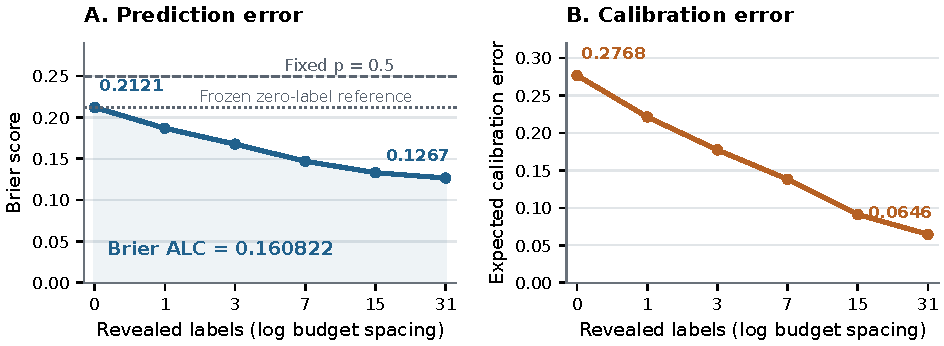
\includegraphics[width=\linewidth]{figures/learning_curves.pdf}
\caption{Pair macro means from the supplied scoring tables. The Brier curve improves at every checkpoint. The dotted reference freezes each target's zero-label prediction at all later budgets; the dashed reference always predicts 0.5. The shaded area represents the normalized learning-curve calculation up to its constant axis-width factor. ECE is a separate calibration diagnostic.}
\label{fig:macro}
\end{figure}

\begin{table}[H]
\centering
\caption{Aggregate results. Each row averages the same nine subject--benchmark pairs equally.}
\label{tab:budget}
\small
\begin{tabular}{@{}rrrrr@{}}
\toprule
Labels & ALC weight & Mean Brier & Mean ECE & Brier gain from zero \\
\midrule
0  & 0.10 & 0.212061 & 0.276844 & 0.000000 \\
1  & 0.20 & 0.186937 & 0.221364 & 0.025124 \\
3  & 0.20 & 0.167660 & 0.177372 & 0.044401 \\
7  & 0.20 & 0.146991 & 0.138118 & 0.065070 \\
15 & 0.20 & 0.133155 & 0.091226 & 0.078906 \\
31 & 0.10 & 0.126671 & 0.064634 & 0.085390 \\
\bottomrule
\end{tabular}
\end{table}

\paragraph{Magnitude of adaptation.}
Mean Brier error decreases by 0.085390 from zero to 31 labels, or 40.27\% relative to the zero-label value. Seven labels capture 76.20\% of that observed endpoint gain; fifteen capture 92.41\%. The first few responses therefore carry substantial practical value. Later checkpoints continue to improve the average, with diminishing mean reduction per additional label.

\paragraph{Two transparent references.}
The fixed-0.5 reference has Brier ALC 0.25, so the ensemble's reported ALC is 35.67\% lower. This is an arithmetic reference that requires only binary outcomes. A second reference holds each target's initial prediction fixed throughout evaluation. Its learning curve is flat at the observed zero-label Brier mean, 0.212061. Against that reference, observed adaptation reduces ALC by 0.051239, or 24.16\%. These transparent references quantify the value of the forecast and its adaptation using the same recorded response set.

\paragraph{Aggregation matters.}
Weighting the nine pair ALCs by their displayed distinct-item counts instead gives 0.159046. That diagnostic changes the weighting rule and differs from the official score. We consistently report the equal-weight pair mean. We also preserve the distinction between 496 unique subject--item pairs and the response-level denominator used inside each pair's Brier calculation.
